\section{Methodology}
\subsection{Where do we look ?}
We want to compare the proportion and the quantity of renames detected by git in this 3 pieces of the software:\\
The Maintenance part, the Development part and the Initialisation part. Plus we want to divide the Development part by major releases.\\
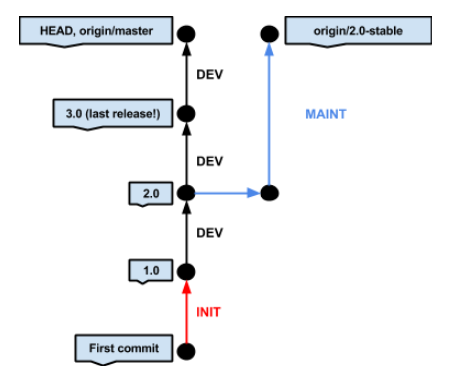
\includegraphics[scale=0.5]{illustrations/draw1}\\
Three types:\\
\textbf{MAINT:} Caintenance branch, a branch which has its head out of master branch. Only commits which are reachable from the branch and not from master.\\
\textbf{INIT:} Commits from the first one (included) to the first major release tag on branch master.\\
\textbf{DEV:} Commits between this major release tag to the next one on branch master.\\
\textbf{(last release!):} commits from the last major release tag to HEAD.\\
\label{subsec:Where do we look ?}
\subsection{Measures}
We will define here the measure we want to observe on the history of the projects creation.\\\\	
\textbf{\# of files :} number of files in the whole project at the head of branch , respectively end of release (=beginning to next release)\\
\textbf{\# of active files:} number of files active (=created or deleted or copied or modified or renamed) in this branch, resp. release.\\
\[ \textbf{\% of active files} = \frac{\# of active files}{\# of files} \times 100 \] \\
\textbf{\# of modifications:}  number of modifications (=create, delete, copy, rename, modif) on files recorded in the branch, resp. release.\\
\textbf{\# of renames:} number of renames recorded on the branch, resp. release\\
\[ \textbf{\% of renames} = \frac{\# of renames}{\# of modifications} \times 100 \] \\
\[ \textbf{\% of files renamed} = \frac{\# of active files renamed}{\# of files} \times 100 \] \\
this give us the proportion of all files in the project renamed in this branch, resp. release and shows its impact on the whole project.\\
\[ \textbf{\% of active files renamed} = \frac{\# of active files renamed}{\# of active files} \] \\
this give us the proportion of active files in the branch, resp. release, renamed in the branch, resp. release. So ''\% of active files renamed'' $\geq$ ''\% of files renamed''. \\
\label{subsec:Measures}

\subsection{Process}

We will describe here the process to follow to obtain this numbers considering any git repository which follows our model. A Ruby script implementation of the following process is given in annexe.\\
First of all we need to list major releases tags in a chronological ascending order. This part can not be automated because of the different tag conventions between projetcs like:
\begin{itemize}
\item PHPunit: 3.5.0, 3.6.0 etc. 
\item Pyramid: 1.0, 1.1 etc.
\item Jenkins: jenkins-1\_400,  jenkins-1\_410 etc.
\item Rails: v2.0.0, v2.1.0 etc. 
\end{itemize}
\medskip
Begin the process:\\
We list the project remotes branches. Browsing the branches, all of them we be considered as maintenance branch except origin/master, the initial and developement branch. Most of the time, specific maintenance branches are followed by “stable”. But if the branch is listed here, it means it has it’s head out of master branch and so it is a maintenance branch since its last merge with master.\\\\
The work is divided in two major step:
\begin{itemize}
\item The maintenance branches
\item origin/master
\end{itemize}
\medskip
If the branch is origin/master, the work will be divided again in:
\begin{itemize}
\item first commit(included) to first release tag
\item fisrt tag to last tag (one release after another)
\item last tag to HEAD
\end{itemize}
\medskip
So in any of the four conditions, we will generate the git log between revision range.
The major part of the work will be on this commits log. We choosed to work on a general log more than mining the history of every files one after the other for performance reasons. Especially on big projects (rails, jenkins). Moreover this technique only works for the files alive at the HEAD of the project and not from one previous revision. So we analyse all the log in one block, with the good command and options it contains enough informations. Log lines stored in simple structures like arrays, we can easily count modifications or renames detected.\\
We will also need to get all the alive files at the end of the log, at the second revision range (branch head or the end of one release).\\\\
Then the principal algorithm will browse the log :\\
Browsing the log in a chronological order will allow us to follow the renames or modifications and rebuilt the history of files.
The typical rename in the log looks like ''rename bob/\{henry $\Rightarrow$ josef\}/george.py (86\%)''
As exemple, if ''bob/henry/george.py'' is already recorded, we need to follow ''bob/josef/george.py'' instead in the renames and modifications record.
There is some other cases to consider, for exemple ''\{henry $\Rightarrow$ \}'' or without ''\{'' or the ''copy'' etc.\\
Each files recorded are unique and only the last name of renamed files is considered.
We finally need exclude all the files deleted before the end of the commits log comparing with the list of alive files at the end of the revision range calculated earlier.\\ 	
\label{subsec:Process}
		
\label{sec:methodology}
